% !TEX TS-program = pdflatex
% !TEX encoding = UTF-8 Unicode

% This is a simple template for a LaTeX document using the "article" class.
% See "book", "report", "letter" for other types of document.

\documentclass[11pt]{article} % use larger type; default would be 10pt.
\setcounter{secnumdepth}{2}

\usepackage{paralist} % very flexible & customisable lists (eg. enumerate/itemize, etc.)

\usepackage[utf8]{inputenc} % set input encoding (not needed with XeLaTeX)
\usepackage{float} % to place float images correctly
\usepackage{color} % to color text
\usepackage{enumitem} % for lists
\usepackage{subfigure} % for mockups
\usepackage[font={it}]{caption} % for captions

%%% Examples of Article customizations
% These packages are optional, depending whether you want the features they provide.
% See the LaTeX Companion or other references for full information.

%%% PAGE DIMENSIONS
\usepackage{geometry} % to change the page dimensions
\geometry{a4paper} % or letterpaper (US) or a5paper or....
% \geometry{margin=2in} % for example, change the margins to 2 inches all round
% \geometry{landscape} % set up the page for landscape
%   read geometry.pdf for detailed page layout information

\usepackage{graphicx} % support the \includegraphics command and options

% \usepackage[parfill]{parskip} % Activate to begin paragraphs with an empty line rather than an indent

\usepackage{listings}
\usepackage{color}
 
\definecolor{codegreen}{rgb}{0,0.4,0}
\definecolor{codegray}{rgb}{0.5,0.5,0.5}
\definecolor{codepurple}{rgb}{0.58,0,0.82}
 
\lstdefinestyle{mystyle}{ 
    commentstyle=\color{magenta},
    keywordstyle=\color{blue}\bfseries,
    numberstyle=\tiny\color{codegray},
    stringstyle=\color{codepurple},
    basicstyle=\footnotesize,
    breakatwhitespace=false,         
    breaklines=true,                 
    captionpos=b,                    
    keepspaces=true,                 
    numbers=left,                    
    numbersep=5pt,                  
    showspaces=false,                
    showstringspaces=false,
    showtabs=false,                  
    tabsize=2,
   emph={self}, 
   emphstyle=\color{blue}, 
   emph={[2] BookingManager, FineManager}, 
   emphstyle=[2]\color{codegreen}\bfseries, 
   emph={[3]__init__, newBook, removeReservation, getReservation, manageExpired, min_heap, pop, now, timedelta, expireReservation}, 
   emphstyle=[3]\color{codegreen}, 
}
 
\lstset{style=mystyle}





%%% PACKAGES
\usepackage{booktabs} % for much better looking tables
\usepackage{array} % for better arrays (eg matrices) in maths
%\usepackage{paralist} % very flexible & customisable lists (eg. enumerate/itemize, etc.)
\usepackage{verbatim} % adds environment for commenting out blocks of text & for better verbatim
\usepackage{subfig} % make it possible to include more than one captioned figure/table in a single float
% These packages are all incorporated in the memoir class to one degree or another...

%%% HEADERS & FOOTERS
\usepackage{fancyhdr} % This should be set AFTER setting up the page geometry
\pagestyle{fancy} % options: empty , plain , fancy
\renewcommand{\headrulewidth}{0pt} % customise the layout...
\lhead{}\chead{}\rhead{}
\lfoot{}\cfoot{\thepage}\rfoot{}

%%% SECTION TITLE APPEARANCE
\usepackage{sectsty}
\allsectionsfont{\sffamily\mdseries\upshape} % (See the fntguide.pdf for font help)
% (This matches ConTeXt defaults)

%%% ToC (table of contents) APPEARANCE
\usepackage[nottoc,notlof,notlot]{tocbibind} % Put the bibliography in the ToC
\usepackage[titles,subfigure]{tocloft} % Alter the style of the Table of Contents
\renewcommand{\cftsecfont}{\rmfamily\mdseries\upshape}
\renewcommand{\cftsecpagefont}{\rmfamily\mdseries\upshape} % No bold!



\usepackage{listings}
\usepackage{pxfonts}

%%% END Article customizations

%%% The "real" document content comes below...




\title{Apache OFBiz: Code Inspection of Selected Classes \\ {\Large Version 1.0}}
\author{Simone Mosciatti \& Sara Zanzottera}


\begin{document}

\begin{titlepage}

\newcommand{\HRule}{\rule{\linewidth}{0.5mm}} % Defines a new command for the horizontal lines, change thickness here
\center % Center everything on the page

%	LOGO SECTION

\includegraphics[width=10cm]{../DOC/polimiLogoNome.png}\\[0.5cm] % Include a department/university logo
 
%	HEADING SECTIONS
%\textsc{\Large Politecnico di Milano}\\[1cm] % Name of your university/college
%\textsc{\large Software Engineering II} \\
%\textsc{\large A. Y. 2016/2017}


%	TITLE SECTION
%\HRule \\[0.4cm]
\\[2cm]
{ \Huge \bfseries Apache OFBiz:} \\[0.5cm] % Title of your document
{ \LARGE \bfseries Code Inspection of Selected Classes} \\[0.5cm]
{\large Version 1.0}
\\[2cm] 
%\HRule \\[1.5cm]

%	AUTHOR SECTION
\Large \emph{Authors:}\\
{\Large \textsc{Mosciatti}} Simone\\ % Your name
{\Large \textsc{Zanzottera}} Sara\\
\\[1cm]
\emph{Reference Professor:} \\
{\Large \textsc{Mottola}} Luca % Supervisor's Name

\vfill % Fill the rest of the page with whitespace

%	DATE SECTION
{\large January 23, 2017}

\end{titlepage}


\newpage
\tableofcontents
\newpage

\section{Introduction}
This document described the results of a peer review of a few selected classes taken from the Apache OFBiz Project (official website: https://ofbiz.apache.org), an open source product for the automation of enterprise processes that includes framework components and business applications for ERP (Enterprise Resource Planning), CRM (Customer Relationship Management) and other business-oriented functionalities.
 
The code inspection has been carried out following the guidelines described in the reference document provided and consulting the official documentation \\ (https://ofbiz.apache.org/documentation.html) 

\subsection{Reference Documents}
\begin{itemize}
	\item \textit{Code Inspection Assignement Task Description.pdf}
	\item \textit{Code Inspection Assignement Table.xlsx}
	\item Official Documentation of the project at https://ofbiz.apache.org/documentation.html
	\item Source Code of the project at http://mirror.nohup.it/apache/ofbiz/apache-ofbiz-16.11.01.zip
	\item \textit{Brutish Programming} at 
http://users.csc.calpoly.edu/~jdalbey/SWE/CodeSmells/bonehead.html
\end{itemize}


\section{Assigned Classes}

The class assigned to our group is:  \texttt{ {\large MiniLangUtil.java} }  \hfill\\
(\texttt{apache-ofbiz-16.11.01/framework/minilang/src/main/java/org/apache/ \\ 
ofbiz/minilang/MiniLangUtil.java})

\subsection{Role of the assigned class}
This class provides some utility functions for the MiniLang Engine.

Mini-Language is described on the official documentation as follows: \textit{The Mini-Language concept in Open For Business is [...] to create simple languages that simplify complex or frequently performed tasks.}

The specific purpose of this static class is unclear: it simply provides a set of static, utility methods and cannot be instantiated. It includes some fundamental operations, like \texttt{.callMethod()}, that probably needs to not belong to instantiable objects, but are fundamental inside the package.

The documentation does not provide in-depht informations about this section of the OFBiz framework: it is impossible to understand the actual role of the class without a detailed inspection of all the classes of the \texttt{minilang} package.

However, the role of the package itself is clearer, as we can see in the following diagram: it is used as an interpreter for the instructions coming from the Service Engine for the Entity Engine.

\begin{figure}[H]
	\centering
	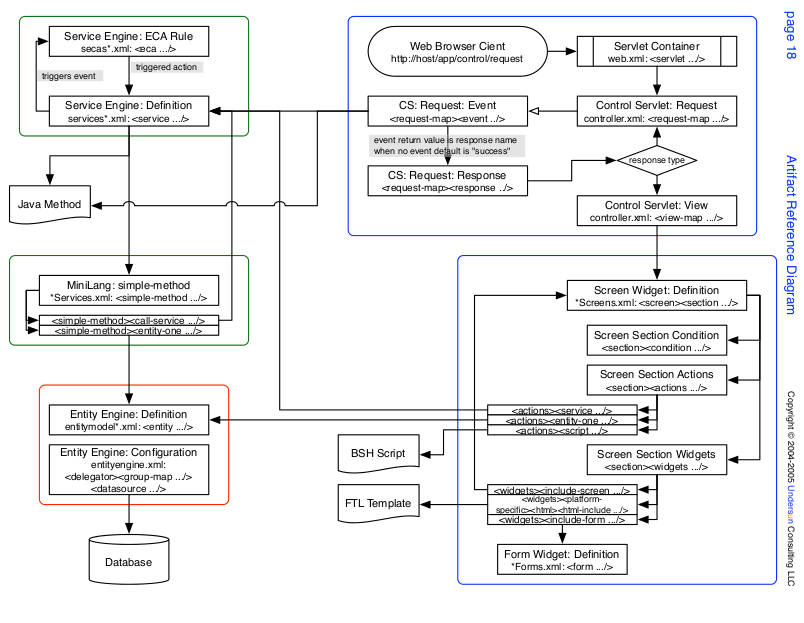
\includegraphics[width=1
\textwidth]{Diagram1.png}
	\caption{OFBiz Artifact Reference Diagram}
\end{figure}


\subsection{Usage of the class}

In order to have a general idea of how and how much the class is used inside the project, we performed a lookup into the repository. \texttt{grep} reports these usages of \texttt{MiniLangUtil} into the OFBiz source code:

\lstinputlisting[language=bash, breaklines=true]{usages2.txt}

Then we check if all methods included in \texttt{MiniLangUtil.java} are actually used in the repo.

\lstinputlisting[language=bash, breaklines=true]{usagesDetail.txt}

The results support our previous hypotesis: \texttt{MiniLangUtil} is an internal class of the \texttt{minilang} package. It is never used outside the package and provides support functions for the processes of the \texttt{minilang} package.

A completely different analysis should be done for the second class included in this source file, \texttt{PlainString}. Such analysis is performed in a dedicated subsection of the next section.


\section{Issues Found}
Issues are listed first concerning the class as a whole, and then method by method.

\subsection{MiniLangUtil class}
\begin{itemize}
	\item Line 60: the public final constant \texttt{module} should be named in capital letters.

	\item Line 65: Sonar reports \texttt{new HashSet<String>()} as a minor issue, because a diamond operator could be used here (\texttt{new HashSet<>()})
	
	\item File organization shows some issues. A lot of lines exceed the 80-char limits, and a few of them (line 111, 152 and 172) exceed the 120-char limit too. In detail, line 111 breaks after char 152 (the total line size is 260 chars), while line 152 reaches the 138 chars and line 172 reaches 124 chars.

	\item Javadoc is inconsistently detailed, and lacks fundamental informations for some methods (see next subsections).

	\item Concerning Java Source Files organization, a peculiar issue has been found. \texttt{MiniLangUtil} includes a public inner class, called \texttt{PlainString}, whose usage and role into the project looks completely different from \texttt{MiniLangUtil}'s ones. See the dedicated section for more details about this issue.

	\item Being an utility class used only inside the package, \texttt{MiniLangUtil} show no need to be a public class. The class definition should be changed from \texttt{public final class MiniLangUtil} into \texttt{final class MiniLangUtil}. 

\end{itemize}

\subsection{containsScript (Line 79)}
\begin{itemize}
	\item Line 80: \texttt{str.lenght()} is called, but \texttt{str} is not guaranteed to be not null. In addition, the method's Javadoc does not says that the behavior of the method in case of null input is a \texttt{NullPointerException} (lacks a \texttt{@throws} statement), while it should be the case.
\end{itemize}

\subsection{autoCorrectOn (Line 96)}
No issues found.

\subsection{callMethod (Line 111)}
\begin{itemize}
	\item This method's Javadoc lacks a lot of informations, starting from parameter's descriptions.
	\item One of the parameters (\texttt{retFieldFma}) has a name that becomes understandable only reading the whole method. It should at least be described in the Javadoc.
	\item Line 133: \texttt{retFieldFma.isEmpty()} is called but \texttt{retFieldFma} is not guaranteed to be not null. Javadoc for this method does not mentions that the result for a null \texttt{retFieldFma} in input is a \texttt{NullPointerException} (lacks a \texttt{@throws} statement)
	\item Line 136: each \texttt{Exception} is caught and changed into a \texttt{MiniLangRuntimeException}. This can be reasonable considering the context (the code simulates a method call), but looks like a code smell.
	\item Line 112-123: Sonar reports this block as a duplicate of lines 92-103 of the method \texttt{CreateObject.exec()}. We believe this block of code should be moved into a separate method and called by both methods at need.
\end{itemize}

\subsection{convertType (Line 152)}
\begin{itemize}
	\item This method's Javadoc lacks a lot of informations, starting from parameter's description.
	\item Line 151: \texttt{@SuppressWarnings} refers to line 172, where an unchecked cast to \texttt{Converter<Object, Object>} is performed. Considering that \texttt{Converters} is a class that belongs to the project (see, at line 38, the \texttt{import} statement) this is probably due to a misunderstanding between developers that are in charge of these classes. \texttt{Converters} should be modified to provide a \texttt{Converter<Object, Object>} in output.
	\item \texttt{==} is often used in place of \texttt{.equals()} to compare objects: see lines 153, 159, 165, 169. These \texttt{==} comparisons should be safe, as they are used only for comparing classes, but as a general rule, it is desirable to use \texttt{.equals()} in any case.
	\item Line 173: the declaration of \texttt{localizedConverted} could be moved into the \texttt{if} block for clarity. The variable is never used outside the block.
	\item Lines 177, 180, 183: Sonar reports the reassigment of new values to some input variables.
	\item This method contains a snippet of code that could be moved elsewhere: lines 182 to 184 looks like input validation for the subsequent call to \texttt{localizedConverter.convert(obj, locale, timeZone, format)}, that would be better located into that method itself.
\end{itemize}

\subsection{flagDocumentAsCorrected (Line 194)}
\begin{itemize}
	\item This method's Javadoc lacks a lot of informations, starting from parameter's description.
	\item Line 195: \texttt{element} is not guaranteed to be not null, but a call to \texttt{element.getOwnerDocument()} is issued. Javadoc for this method does not mention that the result for a null \texttt{element} in input is a \texttt{NullPointerException} (lacks a \texttt{@throws} statement)
\end{itemize}

\subsection{getObjectClassForConversion (Line 211)}
\begin{itemize}
	\item This method's Javadoc, even being a little more detailed that the previous ones, lacks parameter's description and could be a little more detailed about the behavior or the method concerning \texttt{Map, List} and \texttt{Set} classes.
\end{itemize}

\subsection{isConstantAttribute (Line 235)}
\begin{itemize}
	\item Line 236: A call on \texttt{attributeValue.lenght()} is performed, but \texttt{attributeValue} is not guaranteed to be not null. This leads to a peculiar behavior: if \texttt{attributeValue == ""}, it returns \texttt{true}, while if \texttt{attributeValue == NULL}, it throws a \texttt{NullPointerException} (not stated in the Javadoc).
\end{itemize}

\subsection{isConstantPlusExpressionAttribute (Line 251)}
\begin{itemize}
	\item Line 252: A call on \texttt{attributeValue.lenght()} is performed, but \texttt{attributeValue} is not guaranteed to be not null. This leads to a peculiar behavior: if \texttt{attributeValue == ""}, it returns \texttt{true}, while if \texttt{attributeValue == NULL}, it throws a \texttt{NullPointerException}
 (not described in the Javadoc).
	\item Line 254-255: Comments are used in a cryptic way. The statement does not explain why concatenated expressions should be avoided. It does not even contains \texttt{TODO} or \texttt{FIXME} tags.
\end{itemize}

\subsection{isDocumentAutoCorrected (Line 273)}
\begin{itemize}
	\item Line 174: a call to \texttt{document.getUserData()} is issued, but \texttt{document} is not guaranteed to be not null. The consequent  \texttt{NullPointerException} is not even stated in the Javadoc (lacks a  \texttt{@throws} statement).
\end{itemize}

\subsection{writeMiniLangDocument (Line 284)}
\begin{itemize}
	\item This method's Javadoc lacks a lot of informations, starting from parameter's descriptions.
	\item Line 289: the path \texttt{"component://minilang/config/MiniLang.xslt"} is hardcoded. It should be at least moved into a private constant or made configurable by putting it in a config file.
	\item Exceptions management in this method is poor. Twice (line 293 and 310) there is a \texttt{catch(Exception e)} statement that replaces the original exception with a generic error message.
	\item Line 307: \texttt{xmlURL.getFile()} is called, but \texttt{xmlURL} is not guaranteed to be not null. In addition, this statement is put into a \texttt{try \{ \} catch(Exception e)} block that can completely mask this trivial issue.
	\item Line 311: \texttt{xmlURL} is concatenated to the error message string without even checking it for being not null. This can raise a new Exception inside the \texttt{catch} block.
	\item Sonar reports that the whole \texttt{try} block should be replaced with a more compliant "try-with-resources" block, as files are involved. This is an interesting suggestion that should definitely be implemented, but it is not an issue per se.
\end{itemize}

\subsection{PlainString}

\texttt{MiniLangUtil} include a public, inner class called \texttt{PlainString}. This class, which can be found at line 323, is completely empty (the whole source code of \texttt{PlainString} is \texttt{public static class PlainString \{\} }  ) and shows no JavaDoc.

We undestand that creating a specific source file for an empty class like \texttt{PlainString} can be overkill, but anyway this solution is awkward. A public class in general has no reason for being internal, especially into a class like \texttt{MiniLangUtil} that could hold a default modifier instead of the public one.

This solution simply makes difficult for developerd to locate \texttt{PlainString} into the project. 

In addition, being the class empty, we wondered if \texttt{PlainString} is even used into the project, or it is a leftover. So we performed a lookup into the code base to locate eventual usages: the results, shown below, are pretty surprising.

\lstinputlisting[language=bash, breaklines=true]{usagesPlainString.txt}

As we can see, \texttt{PlainString} is user thoughout the whole project, also outside the \texttt{minilang} package. It is even referenced into some \texttt{.xsd} files and into a Groovy script. Seems that \texttt{PlainString} is an entity, probably a field type or something similar, even if the number or references into the codebase (24) seems too low to support the idea \texttt{PlainString} is a fundamental entity for the project.

In addition, the documentation shows no references about \texttt{PlainString}. Also the online version of the Javadoc (found here: https://ci.apache.org/projects/ofbiz/site/ javadocs/org/ofbiz/minilang/MiniLangUtil.PlainString.html) is of no use, as the class itself has no Javadoc.

While it remains unclear why developers should feel the need to use such an empty class to (probably) identify a plain string, and if \texttt{PlainString} is actually the way OFBiz deals with plain strings, the location of this class looks completely wrong.  \texttt{PlainString} should have been located with other basic field types, and into a dedicated Java source file, instead of being a nested class of a randomly chosen class of the project.


\section{Conclusions}

\subsection{Tools used}
During the development of this document we used the following tools:
\begin{itemize}
	\item \textbf{Github} to version control the project
	\item \textbf{\LaTeX} on TeXworks to redact this document
	\item \textbf{SonarQube Scanner 2.8} to double-check the results of the manual code inspection.
\end{itemize}

\subsection{Hours of work}
\begin{itemize}
	\item SZ: 2h on 10/01
	\item SZ: 6h on 11/01
	\item SM: 3h on 12/01
	\item SZ: 7h on 13/01
	\item SZ: 1h on 14/01
	\item SM: 1h on 22/01
	\item SZ: 1h on 23/01
\end{itemize}


\end{document}  
